\documentclass{article}

\usepackage{tikz} 
\usetikzlibrary{automata, positioning, arrows} 

\usepackage{amsthm}
\usepackage{amsfonts}
\usepackage{amsmath}
\usepackage{amssymb}
\usepackage{fullpage}
\usepackage{color}
\usepackage{parskip}
\usepackage{hyperref}
  \hypersetup{
    colorlinks = true,
    urlcolor = blue,       % color of external links using \href
    linkcolor= blue,       % color of internal links 
    citecolor= blue,       % color of links to bibliography
    filecolor= blue,        % color of file links
    }
    
\usepackage{listings}

\graphicspath{ {./images/} }

\definecolor{dkgreen}{rgb}{0,0.6,0}
\definecolor{gray}{rgb}{0.5,0.5,0.5}
\definecolor{mauve}{rgb}{0.58,0,0.82}

\lstset{frame=tb,
  language=haskell,
  aboveskip=3mm,
  belowskip=3mm,
  showstringspaces=false,
  columns=flexible,
  basicstyle={\small\ttfamily},
  numbers=none,
  numberstyle=\tiny\color{gray},
  keywordstyle=\color{blue},
  commentstyle=\color{dkgreen},
  stringstyle=\color{mauve},
  breaklines=true,
  breakatwhitespace=true,
  tabsize=3
}

\newtheoremstyle{theorem}
  {\topsep}   % ABOVESPACE
  {\topsep}   % BELOWSPACE
  {\itshape\/}  % BODYFONT
  {0pt}       % INDENT (empty value is the same as 0pt)
  {\bfseries} % HEADFONT
  {.}         % HEADPUNCT
  {5pt plus 1pt minus 1pt} % HEADSPACE
  {}          % CUSTOM-HEAD-SPEC
\theoremstyle{theorem} 
   \newtheorem{theorem}{Theorem}[section]
   \newtheorem{corollary}[theorem]{Corollary}
   \newtheorem{lemma}[theorem]{Lemma}
   \newtheorem{proposition}[theorem]{Proposition}
\theoremstyle{definition}
   \newtheorem{definition}[theorem]{Definition}
   \newtheorem{example}[theorem]{Example}
\theoremstyle{remark}    
  \newtheorem{remark}[theorem]{Remark}

\title{CPSC-354 Report}
\author{Emma Garofalo  \\ Chapman University}

\date{\today} 

\begin{document}

\maketitle

\begin{abstract}
This report summarizes the key concepts and skills acquired throughout our Programming Languages course, which focused on understanding 
the inner workings of programming languages and designing our own. The course covered a range of topics, including lambda calculus, 
abstract syntax trees, context-free grammars, and term-rewriting systems, as well as the use of theorem provers and parser generators. 
We explored the semantics of functional and imperative languages, the role of mathematical concepts in language design, and how these 
ideas impact practical software development. Through hands-on projects, we gained experience in building interpreters, parsers, and 
reasoning about program correctness. This report provides a week-by-week reflection on the course, demonstrating how theoretical 
concepts in programming languages shape real-world engineering practice and enhance problem-solving skills in software development.
\end{abstract}

\setcounter{tocdepth}{3}
\tableofcontents

\section{Introduction}\label{intro}
This document reflects on the weekly learning journey throughout the Programming Languages course. The primary goal of the course was 
to explore the inner workings of programming languages, understand their foundations, and learn the processes involved in designing and 
implementing them. Rather than focusing on specific programming languages, we were tasked with building one, providing hands-on 
experience with the key concepts that underpin modern language design.

Over the course of the semester, we delved into both theoretical and practical aspects of programming languages. This included studying
the underlying mathematical principles that shape languages, such as lambda calculus, term-rewriting systems, and operational semantics, 
while also learning how to implement these concepts in real-world tools like interpreters, parsers, and theorem provers. Key learning 
objectives involved understanding the structure and behavior of functional and imperative programming languages, as well as mastering the 
techniques required to create parsers using context-free grammars and parser generators like BNFC.

Additionally, we explored how mathematical concepts like abstract data types, proof systems, and the significance of invariants influence 
language design and program correctness. The course also touched on advanced topics like theorem proving and dependent types, offering a 
glimpse into the mathematical foundations of programming and their impact on both practical software development and theoretical computer science.

This document provides a week-by-week breakdown of the course content, outlining the progression from foundational concepts to more advanced 
topics, and reflecting on how these lessons have enhanced our understanding of programming languages and their real-world applications. 
The goal is to highlight not only what we learned, but also how this knowledge can be applied in future programming projects, interviews, 
and further studies in areas such as compiler construction. Ultimately, the course has equipped us with a deeper appreciation for the critical 
role that mathematics and theory play in shaping the tools and languages we use every day in software engineering.
\section{Week by Week}\label{homework}

\subsection{Week 1}
\subsubsection*{Notes}
This week we discussed the foundation of what the class is about.
The main idea was that this class is largely about the intersection
of math and programming, beginning with revisiting the principles we learned
in discrete mathematics. We also learned about LaTeX, which we will be using throughout 
the semester to edit documents like this one. The general idea of the week was setting all of us 
students up for what to expect throughout the semester.

We also covered the topics of Formal Systems, which are explained in more detail in the below
section. And how to determine the relations between a Lean proof and a Math proof.
\subsubsection*{Homework}

The reading that we had to cover for homework discussed the MUI problem, which helps us
break down what a formal system is, and how these attributes can be seen in mathematics like 
discrete math. A formal system carries the requirement of formality, which states that you
must not do anything outside of the set rules. Theorems, axioms, rules of production, and the
decision procedure are all key parts of a formal system.

We also had to complete the tutorial world of the natural number game. 
Here are the solutions for levels 5-8.

\subsubsection*{Level 5}
Goal: a+(b+0)+(c+0)=a+b+c

Solution:
\begin{lstlisting}
rw[add_zero]
rfl
\end{lstlisting}
\subsubsection*{Level 6}
Goal: a+(b+0)+(c+0)=a+b+c

Solution:
\begin{lstlisting}
rw[add_zero c]
rw[add_zero]
rfl
\end{lstlisting}
\subsubsection*{Level 7}
Goal: succ n = n + 1

Solution:
\begin{lstlisting}
rw[one_eq_succ_zero]
rw[add_succ]
rw[add_zero]
rfl
\end{lstlisting}
\subsubsection*{How is this lean proof related to mathematics proofs?:}
The definition of Natural Numbers. 
1. "There is a special natural number, called zero, denoted by 0."
2. "For any natural number n, there is a unique next natural number, called
the successor of n."

\begin{align}
succ n &= n + 1         &   \\
succ n &= n + succ(0)   &    &\text{definition of natural numbers} \\
succ n &= succ(n + 0)   &    &\text{prop. of + for successors} \\
succ n &= succ n        &    &\text{additive identity property} \\
\end{align}
\subsubsection*{Level 8}
Goal: 2 + 2 = 4

Solution:
\begin{lstlisting}
nth_rewrite 2[two_eq_succ_one]
rw[one_eq_succ_zero]
rw[four_eq_succ_three]
rw[three_eq_succ_two]
nth_rewrite 2[two_eq_succ_one]
rw[one_eq_succ_zero]
rw[two_eq_succ_one]
rw[one_eq_succ_zero]
rw[add_succ]
rw[add_succ]
rw[add_zero]
rfl
\end{lstlisting}

I learned a lot from this homework. It basically acted as a refresher for discrete mathematics, and 
how what seems like such a simple solution is much more complicated than you think it is. It also shows 
the various ways that you can derive the same solutions.


\subsubsection*{Comments and Questions}

This week provided me with a good refresher of the discrete mathematics class that I took a while ago. It brought to my attention how much
there is a crossover between math and code, and I am so excited to explore that in this class.

My question for the week relates to the foundation of mathematics, and where it has all evolved from there. We refreshed on discrete math,
which shows us why even the simplest mathematic proofs are valid. And it makes me wonder how mathematics has evolved so much since then. We have
such calculated math that has all built off of these proofs. Seeing how much math has evolved since then, does that mean that math will continue to
evolve in complexity forever? As we create new technologies and understand our world better, will more complicated relationships continue to be found?

\subsection{Week 2: Recursion}
\subsubsection*{Notes}
The main topic of this week was recursion, and how it can be visualized with the "Tower of Hanoi" exercise.
We learned that the definition of recursion is nesting, and variations on nesting. Recursive definitions are
defined in simpler terms of itself, but they never lead to infinite regress or paradox. The "Tower of Hanoi" showed
us this well by demonstrating that once you find a base case (a simpler way to break the problem down), then you can
use that and the successor of that to solve recursively. We considered the problem from the bottom disk up, and observed
how both a stack machine and a rewriting machine can find the efficient recursive solutions.

\subsubsection*{Homework}
The reading that we had for homework was about the "Little Harmonic Labyrinth". This story was a complex example of how
recursion is nesting, and variations on nesting. Another real life example that this reading provided was postponing the 
completion of a task in favor of completing a simpler task, which I think is something that humans naturally do all the time.

We also completed the addition world of the Natural Number Game, and some solutions are outlined below.
\subsubsection*{Level 1}
Goal: 0 + n = n

Solution:
\begin{lstlisting}
induction n with d hd
rw[add_zero]
rfl

rw[add_succ]
rw[hd]
rfl
\end{lstlisting}
\subsubsection*{Level 2}
Goal: succ a + b = succ (a + b)

Solution:
\begin{lstlisting}
induction b with n hn
rw[add_zero]
rw[add_zero]
rfl

rw[add_succ]
rw[hn]
rw[add_succ]
rfl
\end{lstlisting}
\subsubsection*{Level 3}
Goal: a + b = b + a

Solution:
\begin{lstlisting}
induction b with d hd
rw[add_zero]
rw[zero_add]
rfl

rw[add_succ]
rw[hd]
rw[succ_add]
rfl
\end{lstlisting}
\subsubsection*{Level 4}
Goal: a + b + c = a + (b + c)

Solution:
\begin{lstlisting}
induction c with d hd
rw[add_zero]
rw[add_zero]
rfl

rw[add_succ]
rw[hd]
rw[add_succ]
rw[add_succ]
rfl
\end{lstlisting}
\subsubsection*{How is this lean proof related to mathematics proofs?:}
\begin{align}
  a + b + c = a + (b+c)   &      &\text{proof by induction on c} \\
  a + b + 0 = a + (b+0)   &      &\text{base case} \\
  a + b = a + b        &      &\text{additive identity} \\
  succ(a + b + d) = a + (b+succd)&    &\text{inductive step} \\
  succ(a + (b + d)) = a + (b+succd)&      &\text{substitution with inductive hypothesis} \\
  succ(a + (b + d)) = succ(a + (b+d))&      &\text{prop. of + for successors} \\
\end{align}


Then the identity property for addition is performed, showing that a + 0 = a.
Once the base case is proven, the successor must be proven as well.
The property of addition for successors simplifies the goal so that the inductive hypothesis can 
be substituted. With another simplification from the addition of successors, both sides of the equation
are shown to be equivalent.
\subsubsection*{Level 5}
Goal: a + b + c = a + c + b

Solution:
\begin{lstlisting}
induction c with d hd
rw[add_zero]
rw[add_zero]
rfl

rw[add_succ]
rw[add_succ]
rw[hd]
rw[succ_add]
rfl
\end{lstlisting}
This homework was all about recursion. It refreshed my knowledge on how to apply induction
to reach the goal.

\subsubsection*{Comments and Questions}
The "Tower of Hanoi" problem reminded me the give and take when it comes to finding 
recursive solutions. Oftentimes, a recursive solution is a more efficient one, but the time
it takes to think up this solution and the possible complexity of it needs to be taken into consideration.

My question of the week relates to this. Is there a key way to always identify that the most efficient solution to
a particular problem is recursion? I feel like when a problem becomes more complicated, I struggle to identify if 
it can be solved recursively, and because of this, I try multiple other solutions before and waste a lot of time
coming to a recursive solution.

\subsection{Week 3: Programming with LLMs}
\subsubsection*{Notes}
LLMs for literature reviews 

Start discussing creating a calculator in python
\subsubsection*{Homework}

The homework for this week had us focus on how to use LLMs effectively. We had to have
a conversation with an LLM of our choice, and use it to create a literature review
on a topic of our choosing related to programming languages. 

\href{https://github.com/egarof00/CPSC354-HW3}{My literature review}:
I covered the topic of programming languages in video game design. The README is linked in the title above. 
I also wrote a more detailed summary in my discord posting \href{https://discord.com/channels/1277862531226013750/1278164700076707892/1285026014057070632}{here},
under the name MagicTurtle. These documents follow the general trajectory that programming languages have taken over time, and how
they have been used and improved. It also covers the general strengths of the common programming languages used today, and why
they are better for particular types of games than others.

\subsection*{Other Literature Reviews That I Found Interesting:}
\href{https://github.com/keira-ryan/question/blob/main/README.md}{Programming Languages and Art}

Author: Keira Ryan 
As someone who is not as familiar with art, this literature review was very interesting to me.
I think that it took a very good stance on the hot topic of AI art and whether or not
it is "real". It explains that AI can be used as a tool in the art world, and a way to 
experiment with new processes. 

\href{https://github.com/cjoo03/HW3/blob/main/README.md}{Exploring Garbage Collection Across Programming Languages}

Author: Chris Joo
I found this interesting because it is an aspect of programming that is often overlooked.
It is an extremely important part of programming, but when it is taken care of, I often
do not think twice about how it is accomplished. 


\subsubsection*{Comments and Questions}

This week provided me with a good refresher of the discrete mathematics class that I took a while ago. It brought to my attention how much
there is a crossover between math and code, and I am so excited to explore that in this class.

My question for the week relates to the foundation of mathematics, and where it has all evolved from there. We refreshed on discrete math,
which shows us why even the simplest mathematic proofs are valid. And it makes me wonder how mathematics has evolved so much since then. We have
such calculated math that has all built off of these proofs. Seeing how much math has evolved since then, does that mean that math will continue to
evolve in complexity forever? As we create new technologies and understand our world better, will more complicated relationships continue to be found?


\subsection{Week 4: Parsing and Context-Free Grammars}
\subsubsection*{Notes}
Concrete syntax vs. abstract syntax

Parsing

Context-Free Grammar

Caculator with parser generator
\subsubsection*{Homework}

We did various different assignments for homework this week. The first is shown below.
Using this context-free grammar
\begin{lstlisting}
  Exp -> Exp '+' Exp1 
  Exp1 -> Exp1 '*' Exp2              
  Exp2 -> Integer            
  Exp2 -> '(' Exp ')'  
  Exp -> Exp1             
  Exp1 -> Exp2 
\end{lstlisting}
write out derivation/parse trees for each string:
\begin{enumerate}
  \item 2+1
  \item 1+2*3
  \item 1+(2*3)
  \item (1+2)*3
  \item 1+2*3+4*5+6
\end{enumerate}
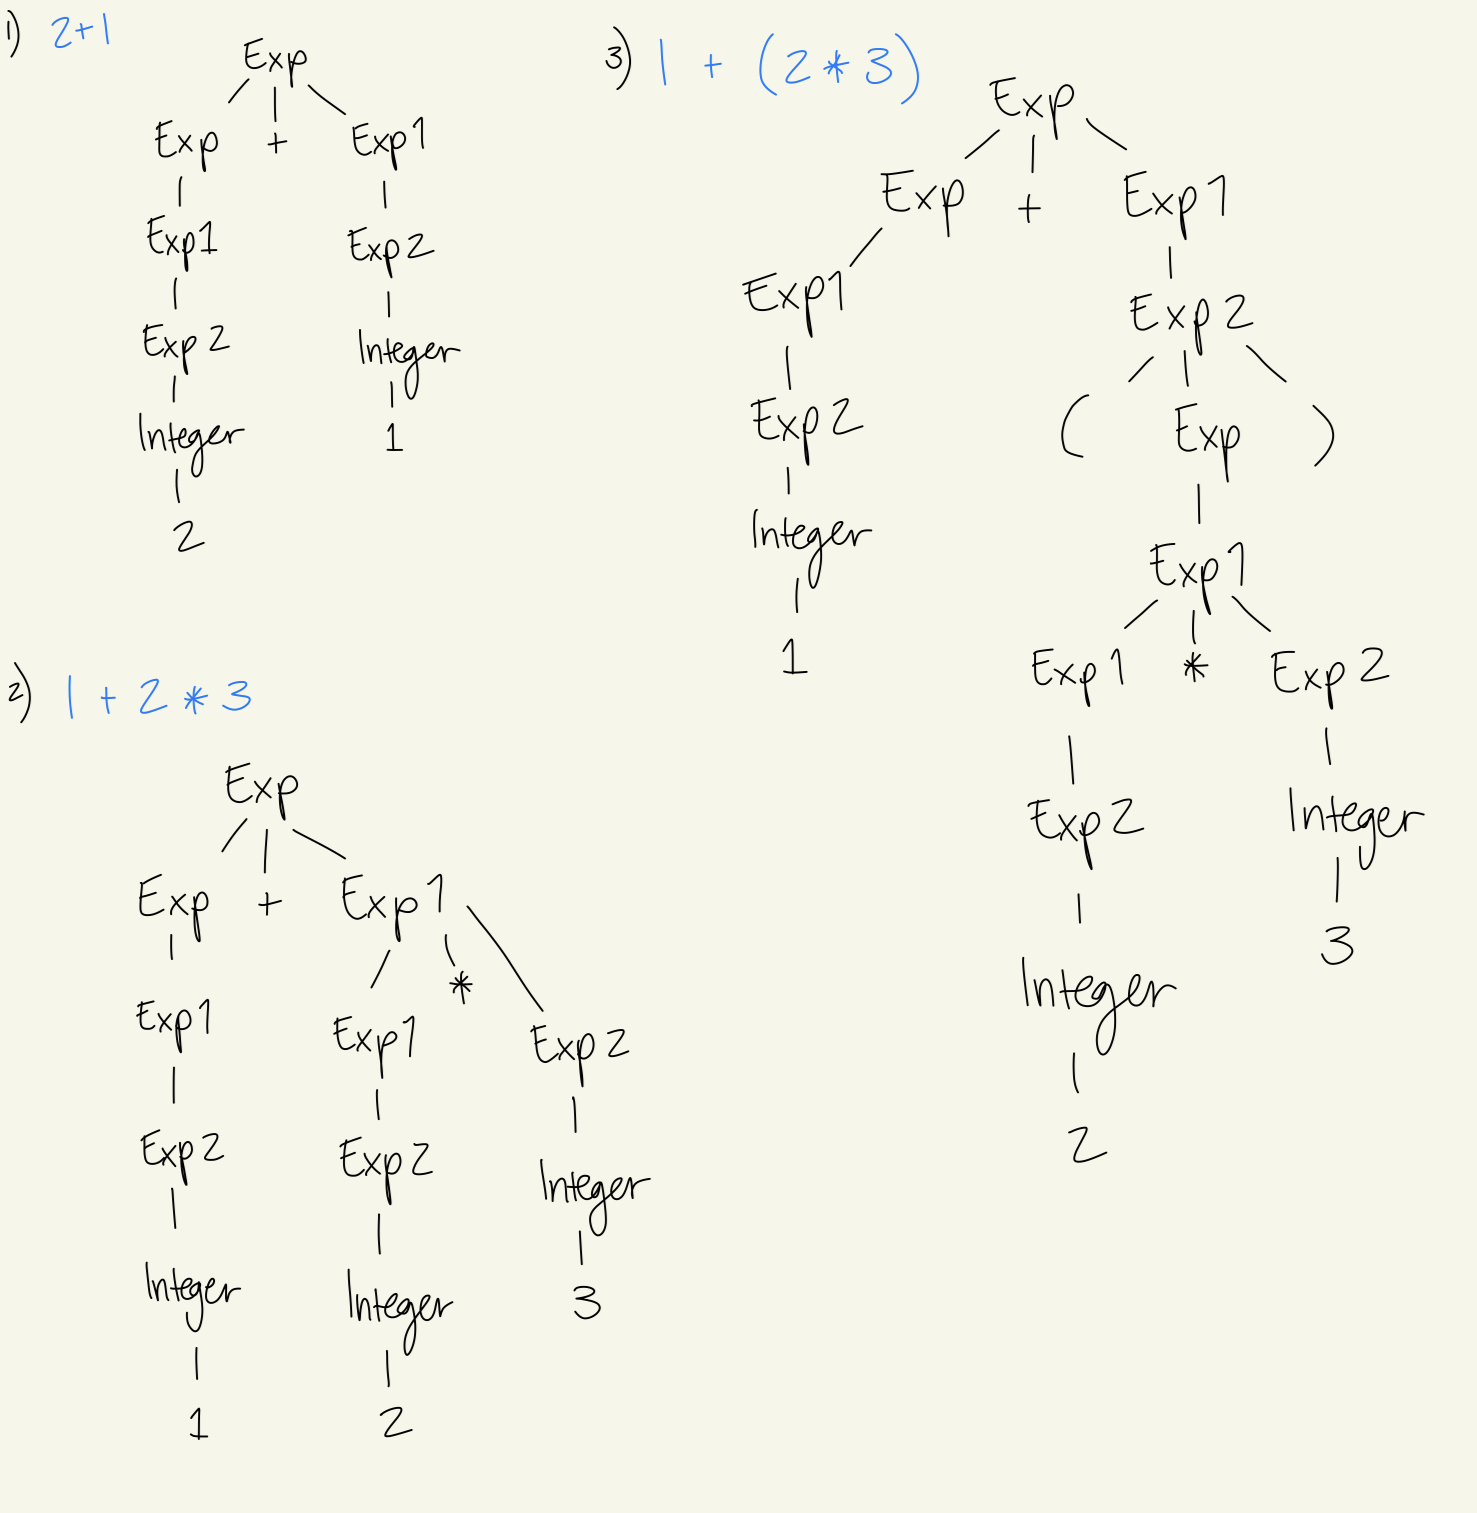
\includegraphics[scale=0.15]{IMG_1712}
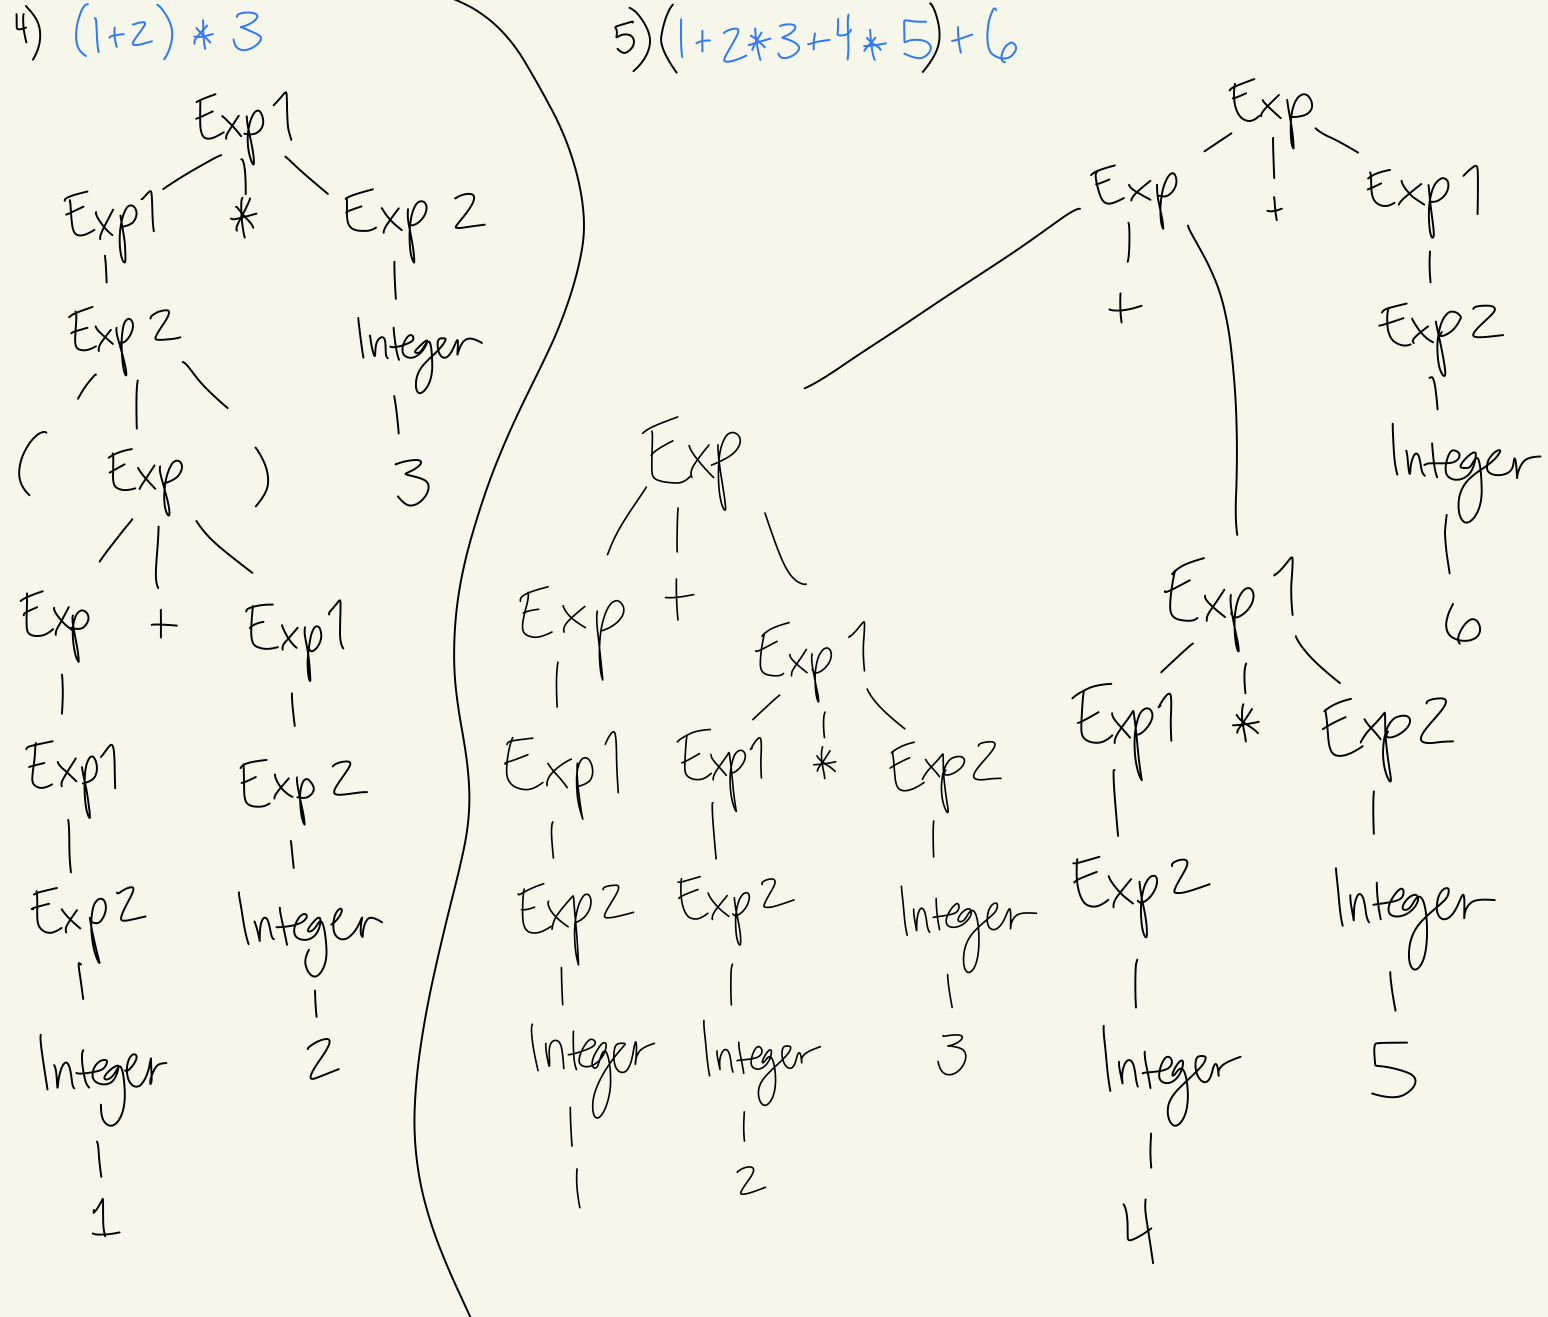
\includegraphics[scale=0.15]{IMG_1713}

We also worked on creating a calculator in python that completes basic math 
operations (parentheses, exponents, multiplication, subtraction, and addition). 
We did this our own way, but we discussed that a great way to complete this project would be 
by creating a parser generator in a software like Lark. 

The reading this week went into detail on the topic of parsing and context free grammars. These context 
free grammars are basically sets of rules that are created to define a language. They must be grammatically 
defined by four components: a finite set of symbols, finite set of variables, a start symbol, and a finite set of
productions. From these, you can perform either recursive inferences or derivations. 
\subsubsection*{Comments and Questions}
This week focused a lot on breaking down what defines a context free grammar and all of the very complicated
details that make up a CFG. The topic puts a lot of focus on what is allowed in a context free grammar, so
I wanted to instead focus on the exclusions from these languages and how they are identified. When a CFG is 
used for a programming language syntax, how is it able to give meaningful error messages? Is it able to 
identify what part of the language that a string would not be valid for and then give an error message in
relation to that? I am just unsure overall of how meaningful error messages are given when a CFG is used
because it is something I have never really thought about until now. 

\subsection{Week 5: Propositions as Types, Dependent Types}
\subsubsection*{Notes}
This week we discussed a LARL (look-ahead, left to right, rightmost derivation parser). This kind of parser
moves all the way to the right when performing a derivation in  order to perform the rightmost derivation first.
In its derivation, it can only perform two actions: shift or reduce. Sometimes this creates shift-reduce conflicts.

\subsubsection*{Homework}
For homework we worked on programming assigment 2, which started with the base of a python calculator script
and lark parsing grammar. Our goal was to add operations to this base while being sure that the order of 
operations was respected, even for long mathematical expressions. For each added expression, we went through the 
steps of adding the operation to the grammar (in the correct order), adding that operation to the python transformer
function, then adding it to the evaluator. Each new operation needed to be tested both on its own and with other
operations in order to ensure that they functioned correctly and respected the order of operations.

We also completed the tutorial world of the Lean Logic Game. This showed how to solve problems in a language
that operates only with variables and functions. No data types or memory exist. The solutions to the tutorial 
world are shown below:
\subsubsection*{Level 1}
\begin{lstlisting}
(P : Prop)(todo_list : P) : P := by
\end{lstlisting}
Solution:
\begin{lstlisting}
  exact todo_list
\end{lstlisting}
\subsubsection*{Level 2}
\begin{lstlisting}
(P S : Prop)(p: P)(s : S) : P /\ S := by
\end{lstlisting}
Solution:
\begin{lstlisting}
  exact <p,s>
\end{lstlisting}
\subsubsection*{Level 3}
\begin{lstlisting}
(A I O U : Prop)(a : A)(i : I)(o : O)(u : U) : (A /\ I) /\ O /\ U := by
\end{lstlisting}
Solution:
\begin{lstlisting}
  exact <<a,i> , o, u>
\end{lstlisting}
\subsubsection*{Level 4}
\begin{lstlisting}
(P S : Prop)(vm: P /\ S) : P := by
\end{lstlisting}
Solution:
\begin{lstlisting}
  exact vm.left : p
\end{lstlisting}
\subsubsection*{Level 5}
\begin{lstlisting}
(P Q : Prop)(h: P /\ Q) : Q := by
\end{lstlisting}
Solution:
\begin{lstlisting}
  exact h.right
\end{lstlisting}
\subsubsection*{Level 6}
\begin{lstlisting}
(A I O U : Prop)(h1 : A /\ I)(h2 : O /\ U) : A /\ U := by
\end{lstlisting}
Solution:
\begin{lstlisting}
  exact <h1.left, h2.right>
\end{lstlisting}
\subsubsection*{Level 7}
\begin{lstlisting}
(C L : Prop)(h: (L /\ (((L /\ C) /\ L) /\ L /\ L /\ L)) /\ (L /\ L) /\ L) : C := by
\end{lstlisting}
Solution:
\begin{lstlisting}
  have h1 := h.left
  have h2 := h.right
  have h4 := h1.right
  have h5 := h4.left
  have h6 := h5.left
  exact h6.right
\end{lstlisting}
\subsubsection*{Level 8}
\begin{lstlisting}
(A C I O P S U : Prop)(h: ((P /\ S) /\ A) /\ -I /\ (C /\ -O) /\ -U) : A /\ C /\ P /\ S := by
\end{lstlisting}
Solution:
\begin{lstlisting}
  have h1 := h.left
  have h2 := h1.left
  have h3 := h1.right
  have h4 := h.right
  have h5 := h4.right
  have h6 := h5.left
  have h7 := h6.left
  exact <h3, h7, h2>
\end{lstlisting}
\subsubsection*{How is this lean proof related to mathematics proofs?:}
\begin{align}
  have h1 := h.left   &      &\text{isolate  (P AND S) AND A} \\
  have h2 := h1.left   &      &\text{isolate P AND S} \\
  have h3 := h1.right        &      &\text{isolate A} \\
  have h4 := h.right&    &\text{isolate I AND (C AND ¬O) AND ¬U} \\
  have h5 := h4.right&      &\text{isolate (C AND ¬O) AND ¬U} \\
  have h6 := h5.left&      &\text{isolate C AND ¬O} \\
  have h7 := h6.left&      &\text{isloate C} \\
  exact <h3, h7, h2>&      &\text{and intro} \\
\end{align}

The goal of this problem is to break down the hypothesis into smaller chunks that are
already known in order to prove that it is true. Once we get to the digestable values
of P AND S, C, and A. We are then able to show that if these are each true individually,
then they can be combined to also all be true.

\subsubsection*{Comments and Questions}
This week we went into parsing trees a bit more in our lecture, and one of the 
things that we talked about were LARLs, or look ahead/rightmost derivation trees.
It is one of the kinds of predictive parsing, but it made me wonder what situations
this type of parsing is actually used, and how it could possibly be flexible in any way. 
Does relying on rightmost derivation limit it's effeciency to very particular problems?
Or is their a way to make it more flexible so that it can handle left-recursive 
grammars just as well?
\subsection{Week 6: Higher Order Functions}
\subsubsection*{Notes}
The topics of this week mostly included currying and lambda calculus. In class, we discussed that currying is like
creating a chain of functions in order to solve a particular problem. This is done because in the scenarios 
that it is used, each function only takes in one argument. 

We also focused a lot of lambda calculus, which as we previously discussed, is made up of only vaiables 
and functions. In order to dive deeper into the topic, we broke it down into syntax and semantics. 
The syntax of lambda caclulus is what I have below. The bottom two being abstraction and application, respectively.
\begin{lstlisting}
  exp -> var
  exp -> 'lambda' var '.' exp
  exp -> exp exp 
\end{lstlisting}

The operational semantics of lambda calculus, otherwise known as how programs will run, was broken down 
when observing the proof of an identity function. We stressed that each function is only able to take
one input, and observing parenthesis properly while using substitution with capture avoiding is necessary
in lambda calculus.
\subsubsection*{Homework}
This week's homework was the "Party Snacks" level of the lean logic world, focusing on lambda calculus. 
We pushed ourselves to solve each problem in a single line. The solutions to problems 1-9 are shown below:
('lambda' and 'maps to' symbols are represented in text because of latex restrictions)
\subsubsection*{Level 1}
\begin{lstlisting}
(P C: Prop)(p: P)(bakery_service : P -> C) : C := by
\end{lstlisting}
Solution:
\begin{lstlisting}
  exact bakery_service p
\end{lstlisting}
\subsubsection*{Level 2}
\begin{lstlisting}
  (C: Prop) : C -> C
\end{lstlisting}
Solution:
\begin{lstlisting}
  exact 'lambda' c 'maps to' c
\end{lstlisting}
\subsubsection*{Level 3}
\begin{lstlisting}
(I S: Prop) : I /\ S -> S /\ I
\end{lstlisting}
Solution:
\begin{lstlisting}
  exact 'lambda' <I, S> 'maps to' <S, I>
\end{lstlisting}
\subsubsection*{Level 4}
\begin{lstlisting}
(C A S: Prop) (h1 : C -> A) (h2 : A -> S) : C -> S
\end{lstlisting}
Solution:
\begin{lstlisting}
  exact 'lambda' c 'maps to' h2 (h1 c)
\end{lstlisting}
\subsubsection*{Level 5}
\begin{lstlisting}
(P Q R S T U: Prop) (p : P) (h1 : P -> Q) (h2 : Q -> R) (h3 : Q -> T) (h4 : S -> T) (h5 : T -> U) : U
\end{lstlisting}
Solution:
\begin{lstlisting}
  exact h5 (h3 (h1 p))
\end{lstlisting}
\subsubsection*{Level 6}
\begin{lstlisting}
(C D S: Prop) (h : C /\ D -> S) : C -> D -> S
\end{lstlisting}
Solution:
\begin{lstlisting}
  exact 'lambda' c d 'maps to' h <c, d>
\end{lstlisting}
\subsubsection*{Level 7}
\begin{lstlisting}
(C D S: Prop) (h : C -> D -> S) : C /\ D -> S
\end{lstlisting}
Solution:
\begin{lstlisting}
  exact 'lambda' <c, d> 'maps to'  h c d
\end{lstlisting}
\subsubsection*{Level 8}
\begin{lstlisting}
(C D S : Prop) (h : (S -> C) /\ (S -> D)) : S -> C /\ D
\end{lstlisting}
Solution:
\begin{lstlisting}
  exact 'lambda' s 'maps to'  <h.left s, h.right s> 
\end{lstlisting}
\subsubsection*{Level 9}
\begin{lstlisting}
(R S : Prop) : R -> (S -> R) /\ (-S -> R)
\end{lstlisting}
Solution:
\begin{lstlisting}
  exact 'lambda' r 'maps to' <'lambda' s 'maps to' r, 'lambda' ns 'maps to' r>
\end{lstlisting}


\subsubsection*{Comments and Questions}
One of the topics generally mentioned this week was the Curry-Howard correspondence.
It demonstrates a connection between formal systems of logic and programming languages,
stating that a propositions correspond to types, proofs correspond to programs, and proof reductions
correspond to program evaluation. It is able to show the direct connections between mathematics 
and programming. My question for the week is how can this understanding improve our approach to
programming?

\subsection{Week 7}
\subsubsection*{Notes}
This week we covered why lambda calculus is turing complete. We wanted to show how to represent
numbers, operations, conditionals, memory, and loops. We also observed recursion in lambda calculus.

\subsubsection*{Homework}
For homework, we had to practice capture avoiding substitution. We were tasked with this problem:

1. Reduce the following lambda term:
\begin{lstlisting}
  ((\m. \n. m n) (\f. \x. f (f x))) (\f. \x. f (f (f x))) 
\end{lstlisting}
Here is my step by step solution to this problem, all using beta reduction:
\begin{lstlisting}
  ((\m. \n. m n) (\f. \x. f (f x))) (\f. \x. f (f (f x))) -> left-most beta reduction
  (\n. (\f. \x. f (f x)) n) (\f. \x. f (f (f x))) -> left-most beta reduction
  (\f. \x. f (f x)) (\f. \x. f (f (f x))) -> left-most beta reduction
  \x. (\f. \x. f (f (f x))) ((\f. \x. f (f (f x))) x) -> right-most beta reduction
  \x. (\f. \x1. f (f (f x1))) (\f. \x2. f (f (f x2))x) -> alpha reduction of x
  \x. (\f. \x1. f (f (f x1))) (\x2. x (x (x x2))x) -> right-most beta reduction
  \x. (\x1. (\x2. x (x (x x2))) ((\x2. x (x (x x2))x) ((\x2. x (x (x x2))x) x1))) -> right-most beta reduction
  \x. (\x1. (\x2. x (x (x x2))) ((\x2. x (x (x x2))x) ((x (x (x x1)))))) -> right-most beta reduction
  \x. (\x1. (\x2. x (x (x x2))) ((x(x(x(x(x(x x1)))))))) -> right-most beta reduction
  \x. (\x1. (x(x(x(x(x(x(x(x(x x1)))))))))) -> right-most beta reduction
\end{lstlisting}
2. Explain what function on natural numbers
\begin{lstlisting}
  (\m. \n. m n)
\end{lstlisting}
implements:

First we need to discuss what church numerals are. In lambda calculus, 
natural numbers are represented as functions because the only two things
that exist in lambda calculus are functions and variables. A church numeral (n)
takes two arguments, a function (f) and a value (x), and applies f to x n times.

In this question, m and n are church numerals. The expression takes two church 
numerals, m and n, as input and returns m as a function and applies n to it. So overall, this function takes two church
numerals, and applies the first church numeral (function) to the second church numeral
(argument), applying the function to the argument.
\subsubsection*{Comments and Questions}
When thinking about church numerals, it adds another layer to lambda calculus that
I didn't really remember needed to be represented. It challenges our understanding of 
the difference between computation and representation in a system that is only able to 
use variables and functions for operations. So, my question for this week is :
In what ways do church encodings in lambda calculus illustrate the relationship between 
data representation and function application, and how might this influence our understanding
of computational efficiency and expressiveness in modern programming languages?
\subsection{Week 8 and 9}
\subsubsection*{Notes}
The focus of week 8 and 9 was on programming assignment 3. The goal was to understand 
how capture avoiding substitution can be implemented into a python script lambda calculus calculator.
It also gave us the opportunity to learn or refresh on how to use the vscode python debugger with 
breakpoints and our own traces to determine where bugs exist within a script.
\subsubsection*{Homework}
As we completed assignment 3, we were told to answer the guiding questions below to help assist us in
understanding the lambda calculus calculator:
\begin{enumerate}
  \item Add new test cases to each of the functions.
  \item Explain why abcd reduces to (((a b) c) d) and why (a) reduces to a.
    \begin{itemize}
      \item The first expression is returned with parenthesis that demonstrate the "order of operations". This
      program evaluates the expressions through leftmost reductions, so abcd is reduced to (((a b) c) d) showing
      that (a b) is first evaluated, then the result is evaluated with c, and then with d. That is why providing the
      program with abcd returns the corresponding answer. (a) reduces to a because there are no further simplifications
      for the given expression.
    \end{itemize}
    \item How does capture avoiding substitution work? How is it implemented?
    \begin{itemize}
      \item Capture avoiding substitution changes the names of variables in an expression with
      alpha substitutions in order to avoid changing nested variables of the same name that are not 
      in the same scope. This is done by renaming variables of the current scope to Var(x), x 
      being the count of substitutions. Doing this maintains proper reductions of the lambda 
      calculus calculator.
    \end{itemize}
    \item Do you always get the expected result? Do all computations reduce to normal form?
    \begin{itemize}
      \item When testing the original program, you do not always get the expected result.
      Any computation that requires rightmost substitution to be completely reduced is not returned 
      with the proper value. 
    \end{itemize}
    \item What is the smallest lambda expression you can find that does not reduce to normal form?
    \begin{lstlisting}
      (\f. \x. f (f x)) (\x. x)
      \end{lstlisting}
    \item Use the python debugger to step through the interpreter (nothing to report for this question)
    \item How does the interpreter evaluate
    \begin{lstlisting}
    ((\m.\n. m n) (\f.\x. f (f x))) (\f.\x. f (f (f x)))
    \end{lstlisting}Write a new line for each substitution.
    \begin{verbatim}
    ((\m.\n. m n) (\f.\x. f (f x))) (\f.\x. f (f (f x)))
    ((\Var1. (\f.\x. f (f x)) Var1) ) (\f.\x. f (f (f x)))
    (\Var1.((\f.(\x.(f (f x)))) Var1))
    ((\Var2.(\Var4.(Var2 (Var2 Var4)))) (\f.(\x.(f (f (f x))))))
    (\Var5.((\f.(\x.(f (f (f x))))) ((\f.(\x.(f (f (f x))))) Var5)))
    \end{verbatim}
    \item Write out the trace in the format that we used for the towers of hanoi for the same
    example as above.
  \begin{verbatim}
    12: eval (((\m.(\n.(m n))) (\f.(\x.(f (f x))))) (\f.(\x.(f x))))
    39: eval ((\m.(\n.(m n))) (\f.(\x.(f (f x)))))
        39: eval (\m.(\n.(m n)))
        44: substitute ((\n.(m n)), ‘m’, (\f.(\x.(f (f x)))))
            89: substitute (substitute((m n), ‘n’, ‘Var1’), ‘m’, (\f.(\x.(f (f x)))))
                92: substitute (‘m’, ‘n’, ‘Var1’)
                92: substitute (‘n’, ‘n’, ‘n’)
                    92: sub substitute (‘m’, ‘m’, ‘m’)
                    92: sub substitute (‘Var1’, ‘m’, (\f.(\x.(f (f x)))))
        45: eval (\Var1.((\f.(\x.(f (f x)))) Var1))
    44: substitute (((\f.(\x.(f (f x)))) Var1), ‘Var1’, (\f.(\x.(f (f (f x))))) )
        92: substitute ((\f.(\x.(f (f x)))), ‘Var1’, (\f.(\x.(f (f (f x))))))
        92: substitute (‘Var1’, ‘Var1’, ‘Var1’)
            89: substitute (substitute((\x.(f (f x))), ‘f’ , ‘Var2’),
            ‘Var1’, (\f.(\x.(f (f (f x))))))
                89: substitute (substitute ((f (f x)), ‘x’, ‘Var3’), ‘f’, ‘Var2’)
                    92: substitute (‘f’, ‘x’, ‘Var3’)
                    92: substitute ((f x), ‘x’, ‘Var3’)
                        92: substitute (‘f’, ‘x’, ‘Var3’)
    92: substitute (‘x’, ‘x’, ‘Var3’)
                            92: substitute (‘f’, ‘f’, ‘Var2’)
                            92: substitute ((f Var3), ‘f’, ‘Var2’)
                                92: substitute (‘f’, ‘f’, ‘Var2’)
                                92: substitute (’Var3’, ‘f’, ‘Var2’)
                                    89: substitute (substitute((Var2 (Var2 Var3)),
                                    ‘Var3’, ‘Var4’), ‘Var1’, (\f.(\x.(f (f (f x))))))
                                        92: substitute (‘Var2’, ‘Var3’, ‘Var4’)
                                        92: substitute ((Var2 Var3), ‘Var3’, ‘Var4’)
                                            92: substitute (‘Var2’, ‘Var3’, ‘Var4’)
                                            92: substitute (‘Var3’, ‘Var3’, ‘Var4’)
                                                92: substitute (‘Var2’, ‘Var1’,
                                                (\f.(\x.(f (f (f x))))))
                                                92: substitute ((Var2 Var4), ‘Var1’,
                                                (\f.(\x.(f (f (f x))))))
                                                    92: substitute (‘Var2’, ‘Var1’,
                                                    (\f.(\x.(f (f (f x))))))
                                                    92: substitute (‘Var4’, ‘Var1’,
                                                    (\f.(\x.(f (f (f x))))))
    45: eval ((\Var2.(\Var4.(Var2 (Var2 Var4)))) (\f.(\x.(f (f (f x))))))
        39: eval (\Var2.(\Var4.(Var2 (Var2 Var4))))\
        44: substitute ((\Var4.(Var2 (Var2 Var4))),’Var2’ , (\f.(\x.(f (f (f x))))))
            89: substitute (substitute((Var2 (Var2 Var4)), ‘Var4’, ‘Var5’), ‘Var2’,
            (\f.(\x.(f (f (f x))))))
      92: substitute (‘Var2’, ‘Var4’, ‘Var5’)
      92: substitute ((Var2 Var 4), ‘Var4’, ‘Var5’)
          92: substitute (‘Var2’, ‘Var4’, ‘Var5')
          92: substitute (‘Var2’, ‘Var4’, ‘Var5’)
              92: substitute (‘Var2’, ‘Var2’, (\f.(\x.(f (f (f x))))))
              92: substitute ((Var2 Var5), ‘Var2’, (\f.(\x.(f (f (f x))))))
                  92: substitute (‘Var2’, ‘Var2’, (\f.(\x.(f (f (f x))))))
                  92: substitute (‘Var5’, ‘Var2’, (\f.(\x.(f (f (f x))))))
        45: eval (\Var5.((\f.(\x.(f (f (f x))))) ((\f.(\x.(f (f (f x))))) Var5)))
  \end{verbatim}
     (we later realized that we did not have to keep a portion of this trace that we accidentally kept but we already went
     through all of it so we decided we might as well leave it in the report.)
\end{enumerate}
\subsubsection*{Comments and Questions}
Week 8 Question: What are the pros and cons of using the Python debugger tool through vscode 
versus print statement debugging?

Week 9 Question: How does the design of Python as a language affect the debugging process of Python scripts?

\subsection{Week 10}
\subsubsection*{Notes}
This week we began discussing the topic of rewriting. We previously defined rewriting as a finite number of 
rules to create finite expressions using pattern matching. We now abstract it even more by removing the 
pattern matching and considering the possibility of an infinite set of rules. We covered directed graphs,
and how they can be used to represent abstract reduction systems (ARSs). We defined confluence to be the ability
to rejoin in rewriting after a divergence, and termination as the ability for the ARS to not admit an infinite
computation. This information was used to set us up for the homework that we have for week 11. 

\subsubsection*{Homework}
For this homework, we were told to reflect on Assignment 3.
Below are the questions we were instructed to answer:
\begin{enumerate}
  \item What did you find most challenging when working through Homework 8/9 and Assignment 3?
    \begin{itemize}
      \item I think the most difficult thing to do was understand the code that already existed for Assignment 3. 
      Taking someone else's code and interpreting it can already be hard, but on top of that we were analyzing code
      for a topic that I am not sure I fully grasped just yet (lambda calculus). I think it was easy for me to understand
      what the program was doing incorrectly, but using that knowledge to find the part of the program that was causing
      the incorrect operation was really difficult for me. This was remedied by what I will discuss in the next
      question. 
    \end{itemize}
    \item How did you come up with the key insight for Assignment 3?
    \begin{itemize}
      \item Once my group talked to Professor Kurz about the issue we were coming across, he gave great insight on a solution
      to help us target the mistake in the program that we needed to fix. He told us to find the smallest example we could that
      was returning an incorrect result. This minimal example was what we really needed to understand what was going on. From there,
      we used the breakpoints that we already established in the code and the python debugger to finally target where we needed to
      put in the missing code and make the program run as intended.
    \end{itemize}
    \item What is your most interesting takeaway from Homework 8/9 and Assignment 3?
    \begin{itemize}
      \item I actually had never used the python debugger before, so understanding that tool was the most interesting 
      thing that I will be able to takeaway from this experience. It will definitely be something that I use in the
      future to help solve coding bugs that I may come across.
    \end{itemize}
\end{enumerate}
\subsubsection*{Comments and Questions}
My question for the week relates to the topic of termination in abstract reduction systems. When evaluating if an ARS
is terminating, is there really any way to determine with absolute certainty that it is? Or are there situations where
it is impossible to identify?
\subsection{Week 11}
\subsubsection*{Notes}
This week was an introduction on rewriting. We covered the definitions of reductions and computations, and 
what an abstract reduction system is. We showed how to model these relationships with directed graphs, and how
to determine if they are confluent, terminating, and if they have unique normal forms. These tools allow us to 
model and create programming language rules.
\subsubsection*{Homework}
We were given ARS questions to complete for homework that are shown below:

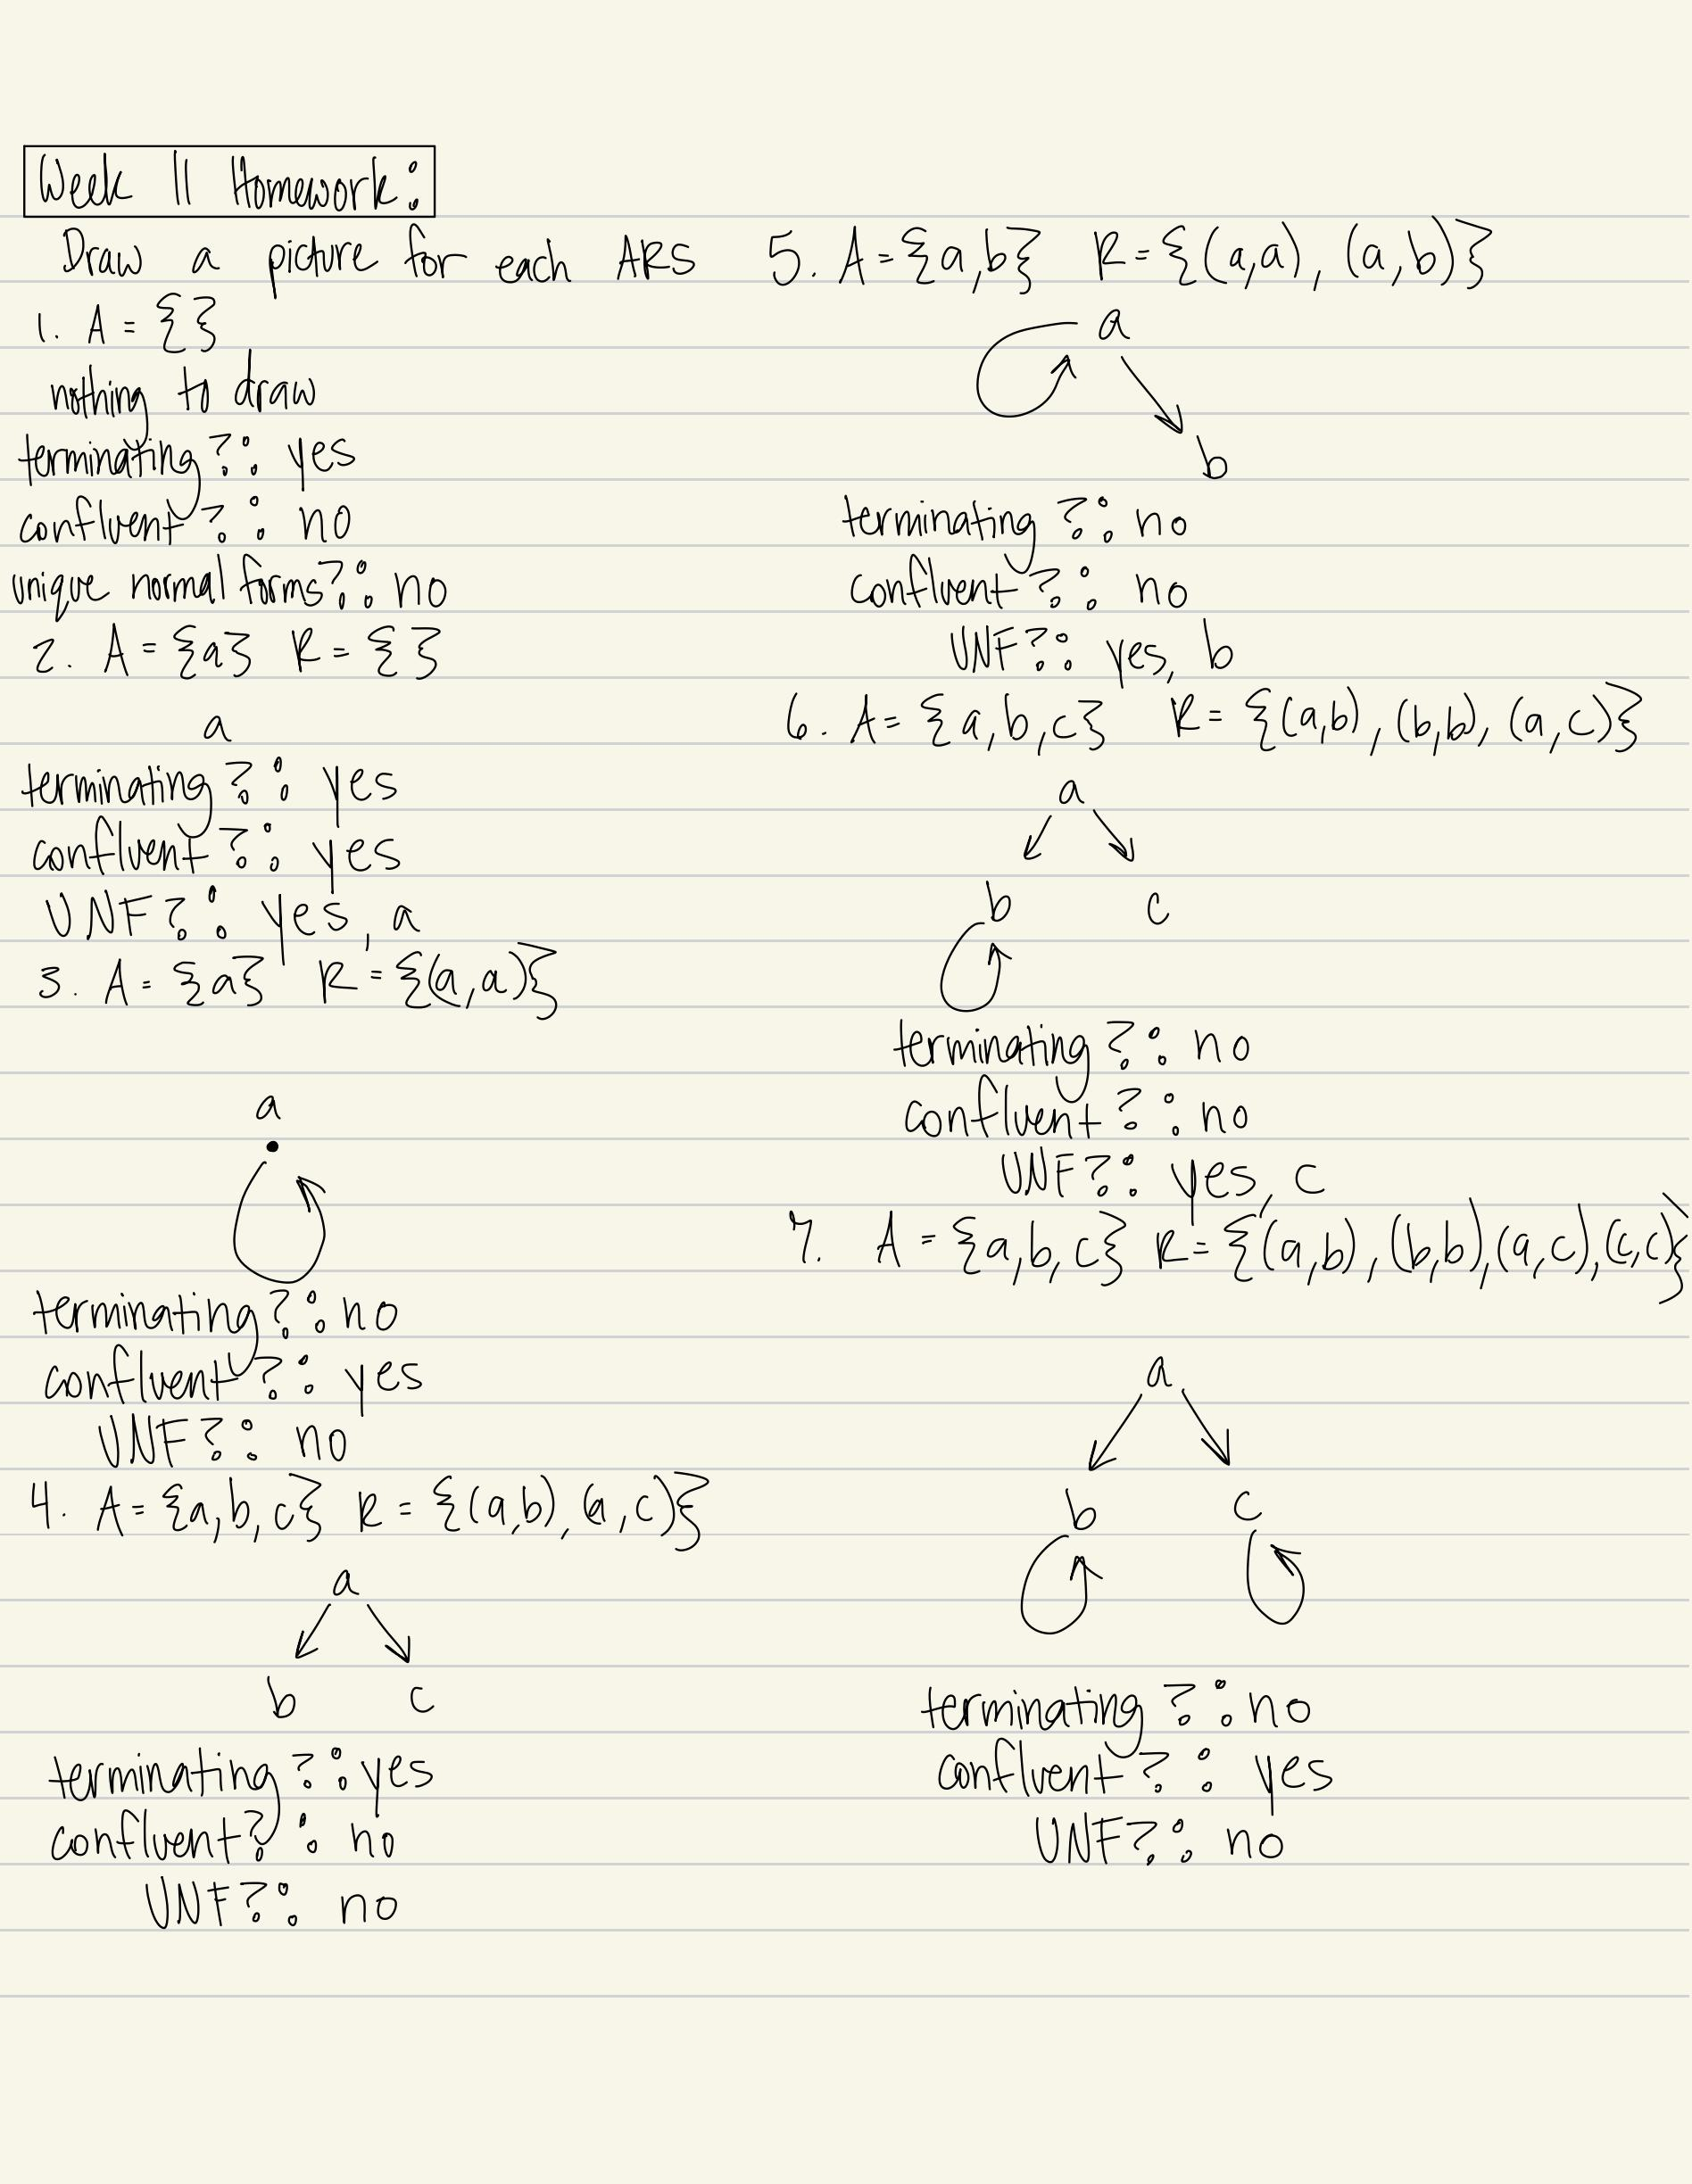
\includegraphics[scale=0.5]{ARS1}
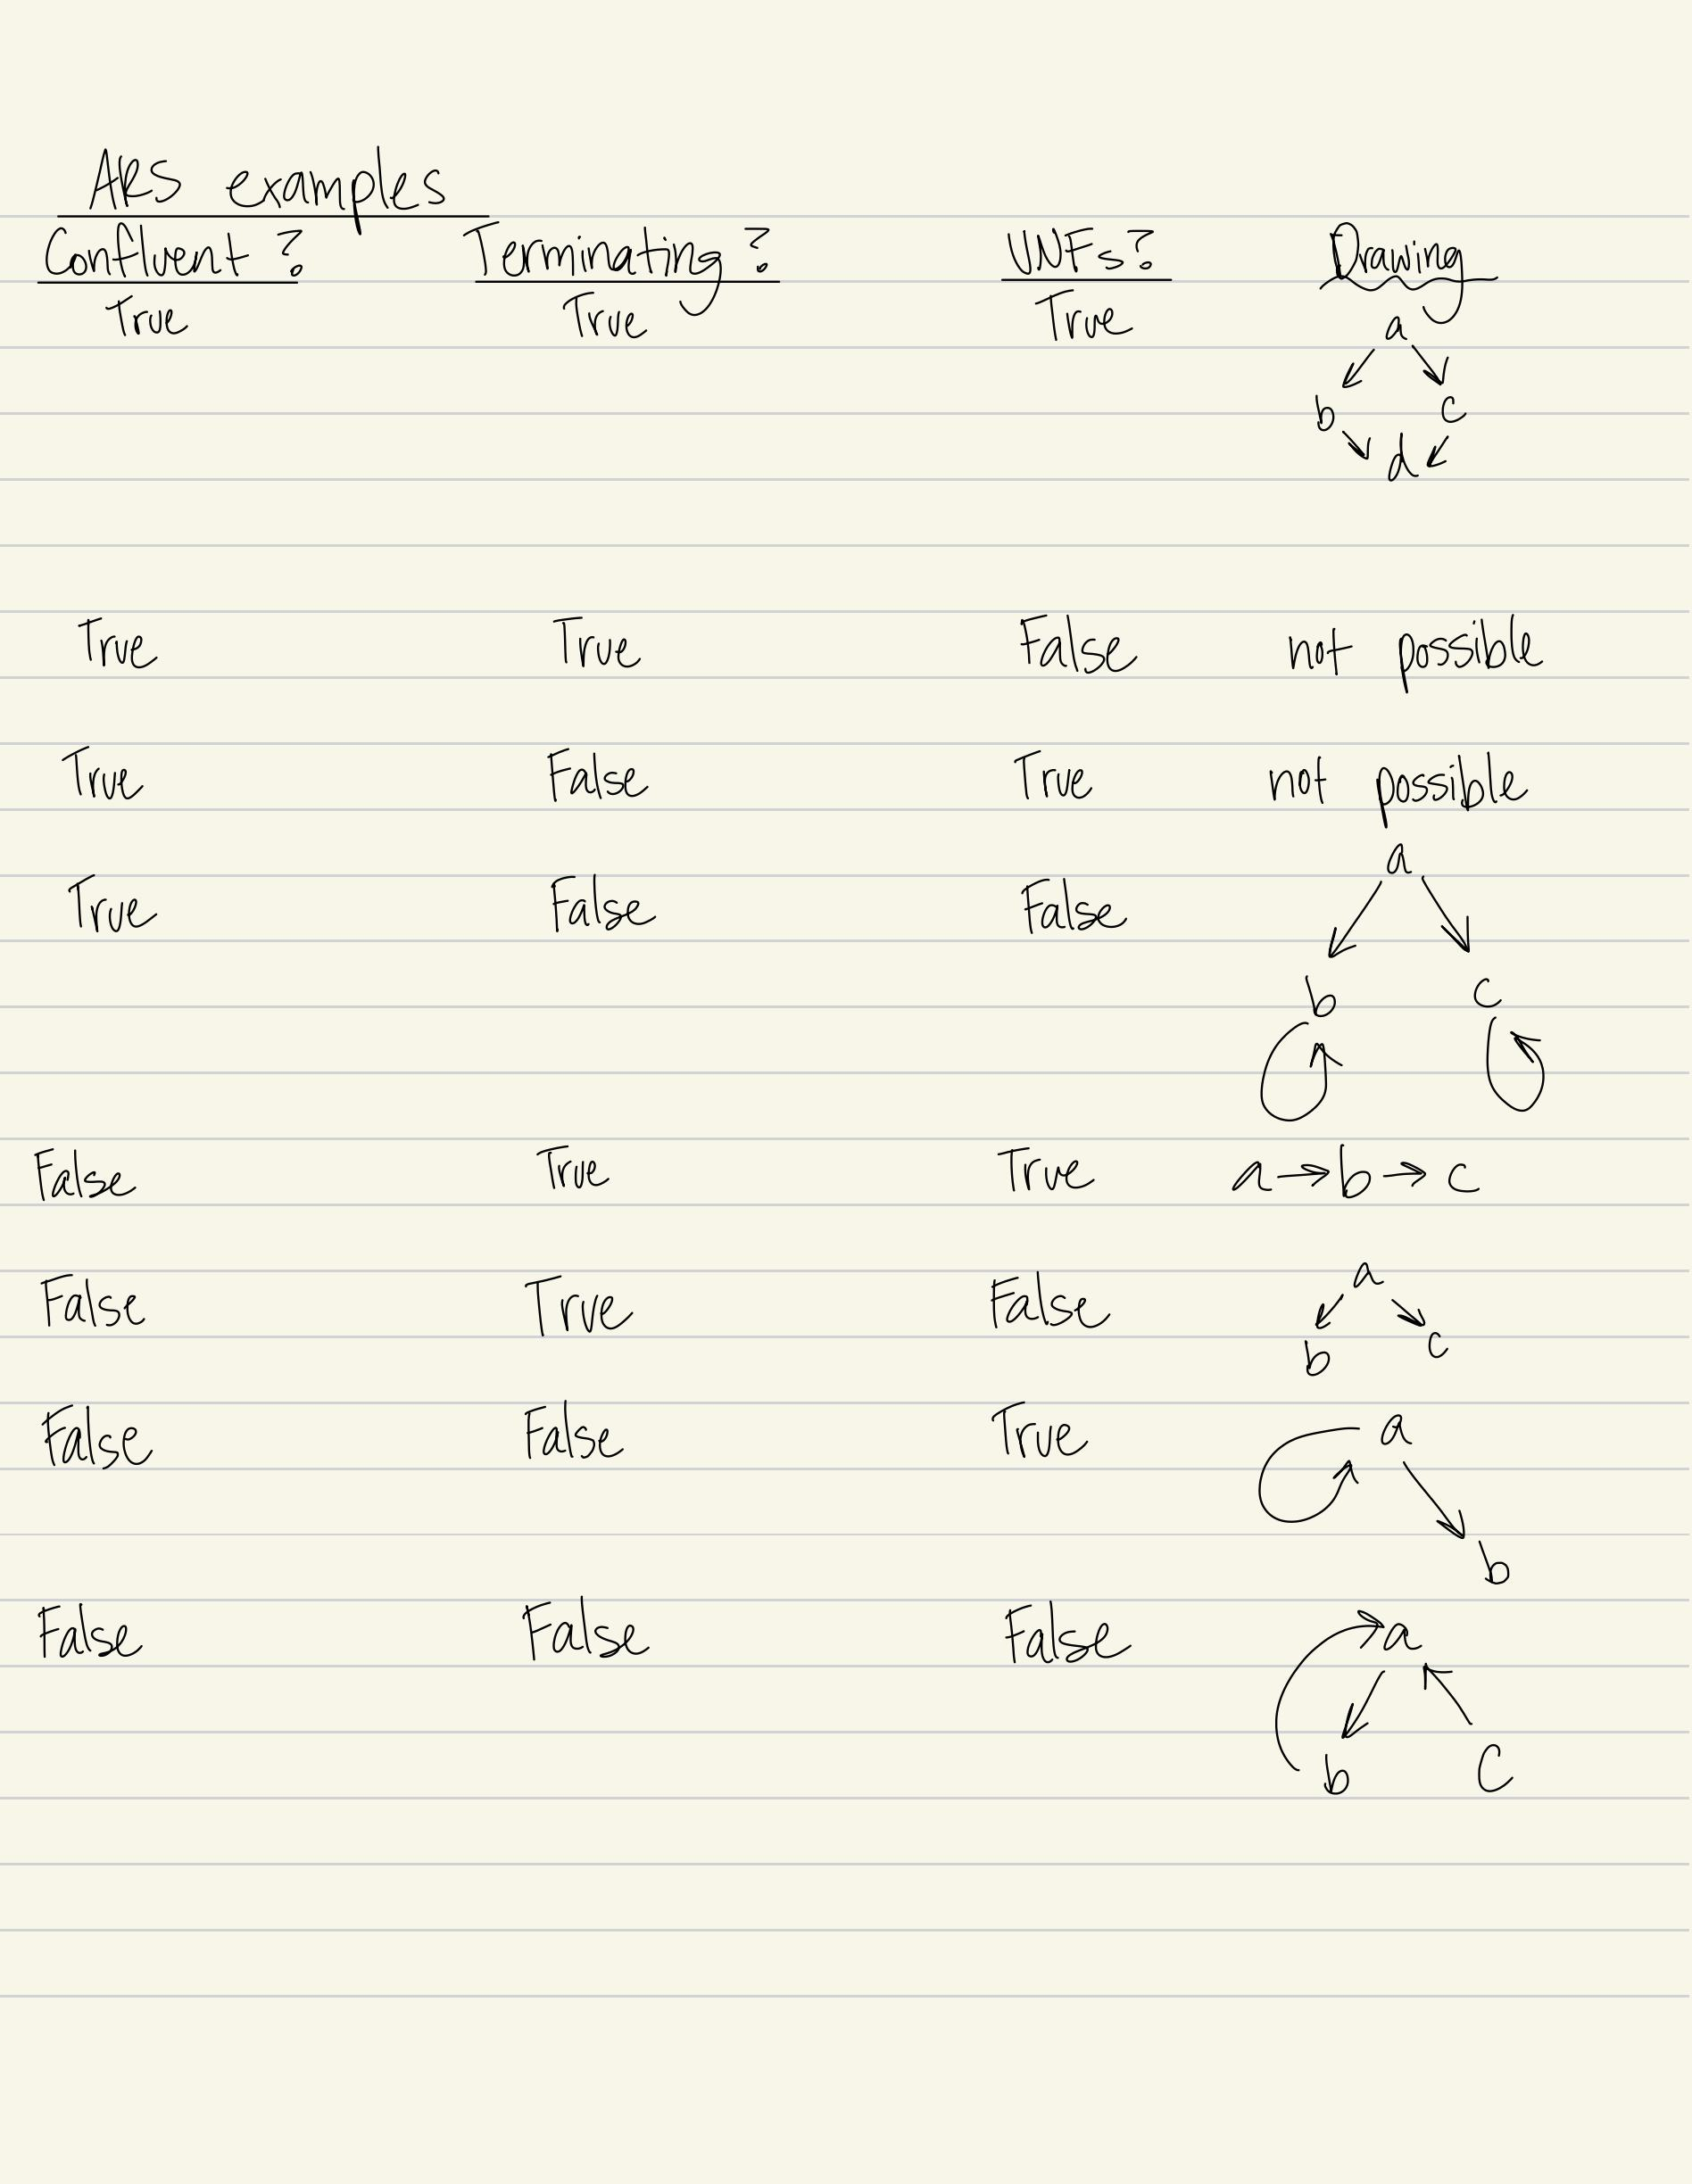
\includegraphics[scale=0.5]{ARS2}
\subsubsection*{Comments and Questions}
My question this week is about confluence. From what we learned and applying it to programming languages,
I feel like confluence is a really important property that can be extremely useful. What would be a situation
where not having confluence is beneficial?
\subsection{Week 12}
\subsubsection*{Notes}
The topic of this week was invariants. We used the example of a sliding puzzle to understand what exactly
they are. We were able to divide the sliding puzzle configurations into solvable and unsolvable, and 
learn that you are unable to travel between these two different categories, so that value is an invariant.
We loosely defined an invairant as something that does not change while the things around it do. We moved
on to discuss the chess puzzle, which was a similar example where we determined that the invariant was that
every tiling covers an equal number of white and black squares. These examples were super interesting to me
and super fun to go over in class. We also worked on implementing recursive behaviour into our lambda 
calculus calculator.
\subsubsection*{Homework}
For homework we had to compute fact 3, which I have done below:

\begin{verbatim}
let rec fact = \n. if n = 0 then 1 else n * fact (n - 1) in fact 3
<def of let>
fact 3 = (\n. if n = 0 then 1 else n * fact (n - 1)) 3
<beta rule: substitute fix F>
if 3 = 0 then 1 else 3 * fact (3 - 1)
<beta rule: substitute 3>
3 * fact (3 - 1)
3 * fact 2
<beta rule: substitute 2>
2 * fact (2 - 1)
2 * fact 1
<beta rule: substitute 1>
1 * fact (1 - 1)
1 * fact 0
<beta rule: substitute 0>
if 0 = 0 then 1 else 0 * fact (0 - 1)
1
<substitute calculated results>
fact 1 = 1 * fact 0 = 1 * 1 = 1
fact 2 = 2 * fact 1 = 2 * 1 = 2
fact 3 = 3 * fact 2 = 3 * 2 = 6
<final result>
fact 3 = 6

\end{verbatim}
\subsubsection*{Comments and Questions}
My question for the week is on invariants. What challenges may arise in a programming
language if it does not have any invariants?
\subsection{Week 13}
\subsubsection*{Notes}
This week focused on a comparison of programming languages. We observed languages like 
LambdaF, OCaml, Python, JavaScript, Rust, Scala, Lean, Racket, and more to look at the 
general similarities and differences in creating a programming language. With this information,
we were able to see how certain languages may perform better in different scenarios. 

We also
discussed the story of "What the Tortoise Said to Achilles". This story is inspired by 
Zeno's Paradox. It is used to challenge ideas in programming languages related to recursion and 
infinite loops. 

The last thing we covered was the black and white hat problem. This was a thought exercise where we were 
given a group of 10 people placed in height order assigned a random hat color that is either white or black. 
Starting at the tallest person in the back of the group (where this individual is able to see everyone in 
front of them), the participants must say what the color of their hat is, and get through the experiment 
with at least 9 correct answers to pass. We were able to create a rule system that the participants would 
follow, tracking the number of remaining white hats and whether that number is even or odd to get at least 
9 correct responses. 
\subsubsection*{Homework}
Rewriting exercises 5 and 5b:

Consider the rewrite rules:
\begin{verbatim}
  ab -> ba
  ba -> ab
  aa ->
  b ->
\end{verbatim}
Reduce some example strings:
\begin{verbatim}
  abba
  baba 
  abba 
  baba 
  baab 
  bb 
  b 
  _
\end{verbatim}
\begin{verbatim}
  bababa
  baabba 
  bbba 
  bba 
  ba 
  a 
\end{verbatim}

Why is this ARS not terminating?
As you can see in the first example, there is the possibility 
of getting stuck in a loop when switching between the ab -> ba 
and ba -> ab rules. Because of the ability to infinitely loop, this
ARS is not terminating. 

How many equivalence classes does it have? Can you describe them in a nice way? What are the normal forms?
Because any instance of b can be removed, the equivalence classes 
depend on the number of a's that are in the string. These strings will 
reduce to either nothing, if there is an even number of a's in the string, or will have a single a 
left in the string if the total number of a's is odd. Any strings with an odd number of a's belong 
in the same equivalence class and any string with an even number of a's belong in the 
same equivalence class. 

Can you change the rules so that the ARS becomes terminating without 
changing the equivalence classes?
The problem rules are the combination of ab -> ba and ba -> ab. We would 
need to remove the possibility of this infinite loop if we wanted to allow 
the ARS to become terminating. The new rules could be:
\begin{verbatim}
  ab -> ba
  ba -> ab
  aa -> 
  b -> 
  ab ->
  ba ->
\end{verbatim}
This would not perform exactly as before though, because bababa would reduce 
to the empty string rather than to a. But the ARS will then have normal forms based off
of the number of a's in the string similarly to before. Any string with the same 
number of a's will reduce to the same normal form.

Write down a question about strings that can be answered using the ARS:
What would be our invariant for this ARS?
In this situation, our invariant would be the number of a's. Depending on their count, the
ARS will always either reduce to the empty string, or to "a".

Consider the rewrite rules:
\begin{verbatim}
  ab -> ba
  ba -> ab
  aa -> a
  b ->
\end{verbatim}
Reduce some example strings:
\begin{verbatim}
  abba
  aba 
  aa 
  a
\end{verbatim}
\begin{verbatim}
  bababa
  baabba 
  babba 
  baba 
  baab 
  bb 
  b 
  _
\end{verbatim}
Why is the ARS not terminating?
This ARS actually is terminating, because every string will eventually 
reach a normal form where no more reductions are possible. 

How many equivalence classes?
Similar to the previous exercise, all b's are removed, so the equivalence 
classes and normal forms depend on the number of a's. Any sequence of a's at all will 
end up reducing to the string "a". If a string just has b's, it will reduce to the 
empty string. So the two equivalence classes are strings that contain any number of 
a's, and strings without a's. Reducing the the two normal forms "a" and "".

Can you change the rules so that the ARS becomes terminating with 
the same equivalence classes?
The ARS is already terminating.

Write down a question about strings that can be answered by the ARS:
What is the benefit of having an ARS that reduces to "a" instead of the empty 
string in as many scenarios (like the exercise previous)? 
\subsubsection*{Comments and Questions}
My question for this week relates to the black and white hat exercise that we 
went over in class. In situations like this, how are you able to tell that there is a 
possible strategy/solution? I feel like we discussed it for an entire hour without having a clear
solution until we wrapped it up at the end, so how are you able to know that you will actually 
arrive at a solution? Like if you changed the order so that the last person to go could see 
everyone's hats and the first person could see none, is there still a possible solution? How 
are you able to realistically deduce if there even will be? 
\section{Lessons from the Assignments}
Throughout this course, I contributed significantly to the group assignments by focusing on various 
aspects of the technical implementation, problem-solving, and application of theoretical knowledge. 
The assignments provided opportunities to integrate both practical and theoretical skills.
\subsection*{Assignment 1: Python Calculator}
This was an individual assignment with the goal of being able to take complicated 
expressions, such as "1+2*3+4*5*6", and returning the correct mathematical output. 
The program needed to be able to evaluate arithmetic expressions, including addition,
subtraction, multiplication, division, and exponentiation. The focus was ensuring that 
all operations were performed in the correct order, including parenthesis. 

The first challenge was implementing a recursive evaluation mechanism. I designed a 
function that would handle parsing using simple precedence rules, multiplication and 
division had higher precedence than addition and subtraction. For example, to evaluate 
3 + 5 * 2, the program would first evaluate 5 * 2 before adding 3, which is the 
expected behavior according to standard operator precedence.

Additionally, in the Parenthesis.py file I developed the error-handling mechanisms 
to deal with incorrect syntax, like mismatched parentheses or invalid operators. 
This was particularly important to ensure that users would receive meaningful 
feedback instead of the program crashing.

The lessons on recursion in the course were directly applicable in this assignment. 
The ability to break down complex expressions into simpler sub-expressions by 
recursive calls made the implementation both efficient and elegant.
\subsection*{Assignment 2: Python Calculator with Lark}
Assignment 2 introduced a new layer of complexity by requiring the calculator to 
parse and evaluate expressions based on a context-free grammar (CFG) defined using 
Lark, a Python library. The task was to define the grammar for arithmetic expressions,
including handling of precedence and associativity, and then implement the evaluation logic.

We began with the ambiguous context-free grammar:
\begin{verbatim}
exp -> exp '+' exp
exp -> exp '*' exp
exp -> exp '^' exp
exp -> exp '-' exp
exp -> '-' exp 
exp -> 'log' exp 'base' exp
exp -> '(' exp ')'
exp -> number
\end{verbatim}
The grammar needed to properly reflect the precedence rules for arithmetic operations, where 
exponentiation should be evaluated before multiplication and division, which in turn should 
be evaluated before addition and subtraction.

The next step was to implement the logic for evaluating these parsed expressions. I built off of a 
class that would recursively traverse the parse tree, evaluating each node based on its type. 
The most interesting challenge in this assignment was ensuring the recursive evaluation respected 
the precedence defined by the grammar. This was not just a matter of following simple rules but also 
ensuring that the AST (abstract syntax tree) was processed in the correct order, which mirrored the 
grammar structure.

This assignment was a good application of the theoretical concepts from lectures, especially the 
lessons on grammars, parsing, and abstract syntax trees. In particular, Lark’s automatic handling 
of parsing allowed me to focus on applying these theoretical concepts in a practical way, saving 
significant time compared to manually building a parser.
\subsection*{Assignment 3: Lambda Calculus Interpreter}
This assignment was a group project that is able to take in lambda calculus statements like 
\begin{verbatim}(\x.x) a\end{verbatim} and return the correct result according to the rules of
lambda calculus. Assignment 3 was a significant leap in complexity. Lambda calculus is a formal 
system used to study computation, and our task was to build an interpreter capable of evaluating 
lambda expressions, which consist of functions and applications.

The primary challenge was implementing beta-reduction, which is the core computation mechanism in lambda calculus. 
The base interpreter program we were given was able to computate some beta-reductions, but had trouble 
evaluating rightmost reductions. Beta-reduction involves replacing the formal parameter of a function with the 
actual argument in the body of the function. I used recursion 
to implement this reduction, applying it to both lambda abstractions and function applications.

This recursive approach to reduction allowed me to handle nested functions and complex expressions efficiently. 
The most valuable takeaway from this project was the practical application of lambda calculus theory, particularly 
the concepts of alpha and beta reduction. By implementing these directly in Python, I was able to gain a deeper understanding 
of how these operations model computation.
\subsection*{Assignment 4: Expanding on Assignment 3}
This assignment continued the group project by extending it to include operations
for sequencing, constructing, and destructing lists. After having the established programs from before, 
we were tasked with adding: 
\begin{verbatim}
prog.       exp -> exp ";;" exp
hd.         exp -> "hd" exp
tl.         exp -> "tl" exp 
nil.        exp -> "#"
cons.       exp -> exp ":" exp
\end{verbatim}
The general sequence of adding in each functionality was to 
\begin{enumerate}
  \item add rule to grammar
  \item update interpreter.py (transformer, evaluate, substitute, linearize)
  \item run tests
  \item repeat
\end{enumerate}
My main contribution to this project was in the expansion of the interpreter’s 
evaluation strategy and implementing the handling of variable environments and scoping.

The key challenge here was ensuring that scoping rules were correctly implemented. Ensuring
that variables defined inside functions or conditionals did not leak into other parts of the program.

This assignment reinforced my understanding of how interpreters work and provided me with a deeper 
appreciation for the complexity of language design, especially the need for managing environments and scope correctly.
\subsection*{Overall Thoughts}
The group assignments and projects provided a rich learning experience, allowing me to apply theoretical 
concepts in a practical setting. From parsing and grammar design in Assignment 2 to the complexities of 
lambda calculus and scoping in Assignment 3 and 4, each task required a deep understanding of both the theory and 
implementation details. My contributions ranged from designing core data structures to implementing recursive evaluation 
mechanisms, all of which were informed by the lectures and course materials. These assignments have significantly deepened 
my understanding of programming languages and computation, preparing me for future challenges in software development and 
language design.
\section{Conclusion}\label{conclusion}
This programming languages course provided a deep dive into both the theoretical foundations and practical applications 
of language design and implementation. The topics covered—recursion, lambda calculus, abstract syntax trees (ASTs), context-free grammars (CFGs)
, parsing, reduction strategies, invariants, and more. And all are integral to the broader field of software engineering, particularly in compiler design, 
language development, and functional programming.

The course emphasized key concepts that are fundamental to understanding how programming languages work under the hood. For example, recursion is not
 just a theoretical concept but a critical mechanism for handling complex data structures and implementing language features like list processing or recursive
function calls. Understanding how recursion works at the core of languages helped me appreciate the elegance and power it provides in both language design
and software development.

Lambda calculus, often referred to as the foundation of functional programming, was another highlight of the course. While the direct application of lambda 
calculus might not be common in everyday software engineering tasks, it deeply influences the design of modern programming languages like Haskell, Scala, 
and even Python (to a certain extent). The principles of lambda calculus inform the development of features such as first-class functions, closures, and 
higher-order functions, all of which are key elements in contemporary programming paradigms.

Abstract syntax trees and context-free grammars were especially useful in understanding how compilers parse and interpret code. The ability to map a program’s 
source code to a tree structure allows compilers and interpreters to analyze and transform code efficiently. Parsing techniques and reduction strategies, like 
beta-reduction in lambda calculus, provide the foundation for designing interpreters and compilers, which are ubiquitous in the software industry. The course also 
touched on important language features such as variables, scopes, and environments, all of which are crucial for building robust, maintainable software.

The most interesting aspect of the course was how it tied theory directly to practical tools. Implementing interpreters and parsers in Python allowed me to 
experience firsthand how abstract concepts like grammars and reduction strategies are realized in code. This hands-on experience is invaluable for anyone 
interested in building compilers or working with domain-specific languages.

My favorite classes were definitely the ones where we attacked puzzles like the chess board puzzle or the white and black hats puzzle. 
Having a unique situation to apply the theories that we are learning about in class to in an interactive environment kept me
interested and allowed me to gain a great understanding of the topics we had already been covering. 

In conclusion, the course offered a rigorous, intellectually rewarding exploration of programming languages. It strengthened my understanding of language 
theory and equipped me with the tools necessary to tackle complex software engineering problems. It also highlighted the importance of both theory and practical 
implementation, an essential aspect of building high-quality, maintainable software.
% \begin{thebibliography}{99}
% \bibitem[BLA]{bla} Author, \href{https://en.wikipedia.org/wiki/LaTeX}{Title}, Publisher, Year.
% \end{thebibliography}

\end{document}
